\documentclass{article}

\usepackage{fancyhdr}
\usepackage{extramarks}
\usepackage{amsmath}
\usepackage{amsthm}
\usepackage{amsfonts}
\usepackage{tikz}
\usepackage[plain]{algorithm}
\usepackage{algpseudocode}
\usepackage{listings}

\usetikzlibrary{automata,positioning}

%
% Basic Document Settings
%

\topmargin=-0.45in
\evensidemargin=0in
\oddsidemargin=0in
\textwidth=6.5in
\textheight=9.0in
\headsep=0.25in

\linespread{1.1}

\pagestyle{fancy}
\lhead{\hmwkAuthorName}
\chead{\hmwkClass\ (\hmwkClassInstructor\ \hmwkClassTime): \hmwkTitle}
\rhead{\firstxmark}
\lfoot{\lastxmark}
\cfoot{\thepage}

\renewcommand\headrulewidth{0.4pt}
\renewcommand\footrulewidth{0.4pt}

\setlength\parindent{0pt}

%
% Create Problem Sections
%

\newcommand{\enterProblemHeader}[1]{
    \nobreak\extramarks{}{Problem \arabic{#1} continued on next page\ldots}\nobreak{}
    \nobreak\extramarks{Problem \arabic{#1} (continued)}{Problem \arabic{#1} continued on next page\ldots}\nobreak{}
}

\newcommand{\exitProblemHeader}[1]{
    \nobreak\extramarks{Problem \arabic{#1} (continued)}{Problem \arabic{#1} continued on next page\ldots}\nobreak{}
    \stepcounter{#1}
    \nobreak\extramarks{Problem \arabic{#1}}{}\nobreak{}
}

\setcounter{secnumdepth}{0}
\newcounter{partCounter}
\newcounter{homeworkProblemCounter}
\setcounter{homeworkProblemCounter}{1}
\nobreak\extramarks{Problem \arabic{homeworkProblemCounter}}{}\nobreak{}

%
% Homework Problem Environment
%
% This environment takes an optional argument. When given, it will adjust the
% problem counter. This is useful for when the problems given for your
% assignment aren't sequential. See the last 3 problems of this template for an
% example.
%
\newenvironment{homeworkProblem}[1][-1]{
    \ifnum#1>0
        \setcounter{homeworkProblemCounter}{#1}
    \fi
    \section{Problem \arabic{homeworkProblemCounter}}
    \setcounter{partCounter}{1}
    \enterProblemHeader{homeworkProblemCounter}
}{
    \exitProblemHeader{homeworkProblemCounter}
}

%
% Homework Details
%   - Title
%   - Due date
%   - Class
%   - Section/Time
%   - Instructor
%   - Author
%

\newcommand{\hmwkTitle}{Assignment 1}
\newcommand{\hmwkDueDate}{September 25, 2021}
\newcommand{\hmwkClass}{Statistical Methods in AI}
\newcommand{\hmwkClassTime}{}
\newcommand{\hmwkClassInstructor}{Professor Anoop Namboodiri}
\newcommand{\hmwkAuthorName}{2019111019}

%
% Title Page
%

\title{
    \vspace{3in}
    \textmd{\textbf{\hmwkClass:\ \hmwkTitle}}\\
    \normalsize\vspace{0.1in}\small{Due\ on\ \hmwkDueDate\ at 12:00 am}\\
    \vspace{0.1in}\large{\textit{\hmwkClassInstructor\ \hmwkClassTime}}
    \vspace{3in}
}

\author{Tushar Choudhary\\
\hmwkAuthorName}
\date{}

\renewcommand{\part}[1]{\textbf{\large Part \Alph{partCounter}}\stepcounter{partCounter}\\}

%
% Various Helper Commands
%

% Useful for algorithms
\newcommand{\alg}[1]{\textsc{\bfseries \footnotesize #1}}

% For derivatives
\newcommand{\deriv}[1]{\frac{\mathrm{d}}{\mathrm{d}x} (#1)}

% For partial derivatives
\newcommand{\pderiv}[2]{\frac{\partial}{\partial #1} (#2)}

% Integral dx
\newcommand{\dx}{\mathrm{d}x}

% Alias for the Solution section header
\newcommand{\solution}{\textbf{\large Solution}}

% Probability commands: Expectation, Variance, Covariance, Bias
\newcommand{\E}{\mathrm{E}}
\newcommand{\Var}{\mathrm{Var}}
\newcommand{\Cov}{\mathrm{Cov}}
\newcommand{\Bias}{\mathrm{Bias}}

\begin{document}

\maketitle

\pagebreak

%%%%%%%%%%%%%%%%%%%%%%%%%%%%%%%%%%%%%%%%%%%%%%%%%%%%%%%%%%%%%%%%%%%%%%%%%%%%%%%%%%%%%%%%%%%%%%%%%%%%%%
%%%%%%%%%%%%%%%%%%%%%%%%%%%%%%%%%%%%%%%%%%%%%%%%%%%%%%%%%%%%%%%%%%%%%%%%%%%%%%%%%%%%%%%%%%%%%%%%%%%%%%
%%%%%%%%%%%%%%%%%%%%%%%%%%%%%%%%%%%%%%%%%%%%%%%%%%%%%%%%%%%%%%%%%%%%%%%%%%%%%%%%%%%%%%%%%%%%%%%%%%%%%%
\begin{homeworkProblem}
    Give an example each of probability mass functions with finite and infinite
ranges. Show that the conditions on PMF are satisfied by your example.

	
    \subsection{Solution}
    

    %We solve each solution algebraically to determine a possible constant
    %\(c\).
    %\\


    %Thus a valid \(c\) is \(c = 2\).
    
    \underline{Finite Range}\\
    \\
For finite range, we can take the example of a Bernoulli distribution.\\
For a real number p such that 0 $<$ p $<$ 1, consider the PMF:
\begin{equation}
    P_{X}(x)=
    \begin{cases}
      1-p, & \text{if}\ x=0 \\
      p, & \text{if}\ x=1 \\
      0, & \text{otherwise}
    \end{cases}
  \end{equation}
 \\
 Here the range of the PMF is R\textsubscript{x} = \{0, 1\} which is finite.\\
 Next, we check whether the conditions of PMF are satisfied by this example
 \begin{equation}
 \begin{split}
     \sum_{x \in R\textsubscript{x}} P_{X}(x) & = P_{X}(0) + P_{X}(1)\\
     & = (1-p) + (p)\\
     & = 1
     \end{split}
 \end{equation}
 \\
 Hence, this is a valid PMF with a finite range.\\
 \\
 \\
\underline{Infinite Range}\\
    \\
For infinite range, we can take the example of a random variable X which represents the number of coin tosses we do till we get the first tails.\\
Consider the PMF:
\begin{equation}
    P_{X}(x)=
    \begin{cases}
      \frac{1}{2^{x}}, & \text{if}\ x \in \mathbb{N} \\
      0, & \text{otherwise}
    \end{cases}
  \end{equation}
 \\
 Here the range of the PMF is R\textsubscript{x} = \mathbb{N} which is infinite.\\
 Next, we check whether the conditions of PMF are satisfied by this example
 \begin{equation}
 \begin{split}
     \sum_{x \in R\textsubscript{x}} P_{X}(x) & = \sum_{x \in \mathbb{N}} P_{X}(x)\\
     & = \sum_{x \in \mathbb{N}} \frac{1}{2^{x}}\\
     & = \frac{1/2}{1-1/2}\\
     & = 1
     \end{split}
 \end{equation}
 \\
 Hence, this is a valid PMF with an infinite range.\\

\end{homeworkProblem}

%%%%%%%%%%%%%%%%%%%%%%%%%%%%%%%%%%%%%%%%%%%%%%%%%%%%%%%%%%%%%%%%%%%%%%%%%%%%%%%%%%%%%%%%%%%%%%%%%%%%%%
%%%%%%%%%%%%%%%%%%%%%%%%%%%%%%%%%%%%%%%%%%%%%%%%%%%%%%%%%%%%%%%%%%%%%%%%%%%%%%%%%%%%%%%%%%%%%%%%%%%%%%
%%%%%%%%%%%%%%%%%%%%%%%%%%%%%%%%%%%%%%%%%%%%%%%%%%%%%%%%%%%%%%%%%%%%%%%%%%%%%%%%%%%%%%%%%%%%%%%%%%%%%%
\pagebreak

\begin{homeworkProblem}
    Show with complete steps that the variance of uniform density is given by equation 10. (Hint: use the expression for variance in equation 5.)
\\

    \solution
    \\
    
    If we have the PDF of a uniform distribution as f_{X}(x) =
    \begin{cases}
      \frac{1}{b-a}, & \text{if}\ a <= x <= b \\
      0, & \text{otherwise}
    \end{cases}
    
    Then required result is \sigma^{2} = \frac{(b-a)^2}{12}. \\
    
    
    We know that for a random variable X, we have \sigma^{2} = $E[X^{2}]-(E[X])^{2}$.\\
    Hence, if we know the values for $E[X^{2}]$ and $E[X]^{2}$ we can calculate the value of $\sigma^{2}$.\\
    \\
    Calculating $E[X]$:
\begin{equation}
\begin{split}
  E[x] & = \int_{a}^{b} \frac{x}{b-a}\,dx\\ 
  & = \frac{1}{b-a}\,\int_{a}^{b} x\,dx\\
  & = \frac{1}{2(b-a)}\,(b^{2}-a^{2})\\
  & = \frac{a+b}{2} 
\end{split}
\end{equation}
Calculating $E[X^{2}]$:
\begin{equation}
\begin{split}
  E[x^{2}] & = \int_{a}^{b} \frac{x^{2}}{b-a}\,dx\\ 
  & = \frac{1}{b-a}\,\int_{a}^{b} x^{2}\,dx\\
  & = \frac{1}{3(b-a)}\,(b^{3}-a^{3})\\
  & = \frac{a^{2}+ab+b^{2}}{3} 
\end{split}
\end{equation}
Calculating $\sigma^{2}$:
\begin{equation}
\begin{split}
  \sigma^{2} & = E[x^{2}] - (E[x])^2 \\
  & = \frac{a^{2}+ab+b^{2}}{3} - (\frac{a+b}{2})^2 \\
  & = \frac{a^{2}+ab+b^{2}}{3} - (\frac{a^{2}+2ab+b^{2}}{4}) \\
  & = \frac{a^{2}+2ab+b^{2}}{12} \\
  & = \frac{(b-a)^2}{12}
\end{split}
\end{equation}
Hence, proved.
\end{homeworkProblem}
%%%%%%%%%%%%%%%%%%%%%%%%%%%%%%%%%%%%%%%%%%%%%%%%%%%%%%%%%%%%%%%%%%%%%%%%%%%%%%%%%%%%%%%%%%%%%%%%%%%%%%
%%%%%%%%%%%%%%%%%%%%%%%%%%%%%%%%%%%%%%%%%%%%%%%%%%%%%%%%%%%%%%%%%%%%%%%%%%%%%%%%%%%%%%%%%%%%%%%%%%%%%%
%%%%%%%%%%%%%%%%%%%%%%%%%%%%%%%%%%%%%%%%%%%%%%%%%%%%%%%%%%%%%%%%%%%%%%%%%%%%%%%%%%%%%%%%%%%%%%%%%%%%%%
\pagebreak

\begin{homeworkProblem}
    Show examples of two density functions (draw the function plots) that have the same mean and variance, but clearly different distributions. Plot both functions in the same graph with different colours.
    \\

    \solution
    \\
    
Consider an exponential distribution with parameter $\lambda$ = 1. The mean of this distribution will be 1/$\lambda$ = 1/1 =1 and variance will be 1/$\lambda^{2}$ = 1/1 = 1.\\

Consider a normal distribution with parameters $\mu$ = 1 and $\sigma$ = 1. The mean of this distribution will be equal $\mu$ = 1 and variance will be equal to $\sigma^{2}$ = 1.\\

Hence, the mean and variance for both these distributions is 1.\\
    
I have written the following code in python3 to generate the graph:
\begin{verbatim}
import matplotlib.pyplot as plt
import numpy as np

x = np.linspace(0, 5, 500, endpoint=True) # 500 points equally distributed from 0 to 4
y1 = np.exp(-x) # Exponential distribution with lambda = 1
y2 = np.exp(-((x-1)**2)/2) / np.sqrt(2*np.pi) # Normal distribution with mu = 1 and sigma = 1
plt.plot(x, y1, label="Exponential Distribution")
plt.plot(x, y2, label="Gaussian Distribution")
plt.legend()
plt.title('Exponential Distribution v/s Gaussian Distribution')
plt.show()
\end{verbatim}

The graph obtained is:
\begin{center}
\begin{figure}[hbtp]
\centering
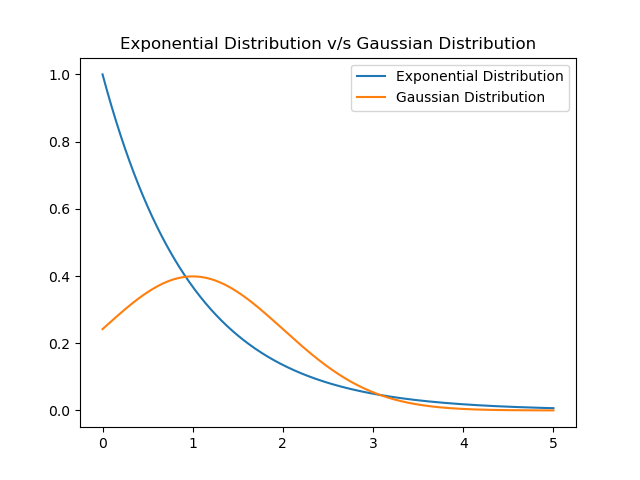
\includegraphics[scale=0.6]{Q3.png}
\caption{Exponential Distribution v/s Gaussian Distribution}
\end{figure}
\end{center}
\end{homeworkProblem}

\pagebreak

\begin{homeworkProblem}
    Show that the alternate expression for variance given in equation 5 holds for discrete random variables as well.
    \\
    
    \solution
    \\
    
    If we have the PMF of a discrete random variable X given by $P_{X}(x)$ over range $R_{X}$, then required result is \sigma^{2} = $E[X^{2}] -E[X]^{2}$. \\
    
    
    We know that for a random variable X, we have \sigma^{2} = $E[(X - E[X])^{2}]$.\\
    \\
    %\sum_{x \in \mathbb{N}} \frac{1}{2^{x}}\\
Calculating $\sigma^{2}$:
\begin{equation}
\begin{split}
  \sigma^{2} & = E[(X - E[X])^{2}]\\
  & = \sum_{x \in R_{x}} P_{X}(x) * (x-E[X])^{2}\\
  & = \sum_{x \in R_{x}} P_{X}(x) * (x^2 - 2xE[X]+E[X]^{2})\\
  & = \sum_{x \in R_{x}} P_{X}(x) x^2 -2E[X] \sum_{x \in R_{x}} P_{X}(x) x + E[X]^{2}\sum_{x \in R_{x}} P_{X}(x)\\
  & = E[X^{2}] -2E[X]*E[X] + E[X]^{2} * 1\\
  & = E[X^{2}] -E[X]^{2}
\end{split}
\end{equation}
Hence, proved.
\end{homeworkProblem}

\pagebreak

\begin{homeworkProblem}
    Prove that the mean and variance of a normal density, N($\mu$,$\sigma^2$) are indeed its parameters, $\mu$ and $\sigma^2$.
    \\

    \solution
    \\
    
    We know that PDF of a normal random variable $X\sim{}N(\mu,\sigma^2)$ is given by $f_X(x)=\frac{1}{\sigma\sqrt{2\pi}}e^{-\frac{(x-\mu)^2}{2\sigma^2}}$. For this distribution, the mean E[X] can be calculated by $E[X] = \int_{-\infty}^{\infty} x f_{X}(x)\,dx$, using which we can get the variance Var(X) = $E[(X-E[X])^{2}]$.\\
    
    Calculating E[X]:
    
    \begin{equation}
    \begin{split}
E[X]&=\int_{-\infty}^\infty xf_X(x)dx\\
&=\int_{-\infty}^\infty\frac{x}{\sigma\sqrt{2\pi}}e^{-\frac{(x-\mu)^2}{2\sigma^2}}dx
\end{split}
\end{equation}
Now in the above equation we will substitute $x=x'+\mu$ to simplify the term, $(x-\mu)^{2}$.\\
Also, d(x) = $d(x'+\mu)$ = dx' (since the mean $\mu$ is constant). The limits shall still stay $-\infty$ to $\infty$.\\
So now we have,\\
\begin{equation}
\begin{split}
E[X]&=\int_{-\infty}^\infty\frac{x'+\mu}{\sigma\sqrt{2\pi}}e^{-\frac{x'^2}{2\sigma^2}}dx'\\
&=\int_{-\infty}^\infty\frac{x'}{\sigma\sqrt{2\pi}}e^{-\frac{x'^2}{2\sigma^2}}dx' + \mu\int_{-\infty}^\infty\frac{1}{\sigma\sqrt{2\pi}}e^{-\frac{x'^2}{2\sigma^2}}dx'
\end{split}
\end{equation}

Now on observing carefully, we can see that the function in the first integral is an odd function and hence its integral from $-\infty$ to $\infty$ will be 0. So we're left with just the second term.

\begin{equation}
\begin{split}
E[X]&= \mu\int_{-\infty}^\infty\frac{1}{\sigma\sqrt{2\pi}}e^{-\frac{x'^2}{2\sigma^2}}dx'\\
&= \mu\int_{-\infty}^\infty f_{X}(x')dx'\\
&= \mu * 1\\
&= \mu\\
\end{split}
\end{equation}
(Using $\int_{-\infty}^\infty f_{X}(x')dx'$ = 1, which is property of probability density function.)
\\
\\
Calculating Var(X):\\

\begin{equation}
\begin{split}
Var(X)&=E[(X-E[X])^2]\\
&=\int_{-\infty}^\infty\frac{(x-E[X])^2}{\sigma\sqrt{2\pi}}e^{-\frac{(x-\mu)^2}{2\sigma^2}}dx\\
&=\int_{-\infty}^\infty\frac{x'^2}{\sigma\sqrt{2\pi}}e^{-\frac{x'^2}{2\sigma^2}}dx'\\
\end{split}
\end{equation}
\\
Since the function inside the above integral is an even function, the value of the integral from $-\infty$ to $\infty$ will be twice the value of value of integral from 0 to $\infty$.
\\
\pagebreak
\\
So we have:

\begin{equation}
\begin{split}
Var(X)&=2*\int_{0}^\infty\frac{x'^2}{\sigma\sqrt{2\pi}}e^{-\frac{x'^2}{2\sigma^2}}dx'\\
\end{split}
\end{equation}

Now in the above function, we substitute $k = \frac{x'^2}{2\sigma^2}$.\\
We have $x'^2$ = $2\sigma^2k$ and from this we can get $dx' = \frac{\sigma dk}{\sqrt{2k}}$.\\
\\
Next,
\\
\begin{equation}
\begin{split}
Var(X)&=2*\int_{0}^\infty\frac{2\sigma^2k}{\sigma\sqrt{2\pi}}\ \ e^{-k} \ \ \frac{\sigma dk}{\sqrt{2k}}\\
&=\frac{2\sigma^2}{\sqrt{\pi}} * \int_{0}^\infty k^{1/2} e^{-k} dk\\
&=\frac{2\sigma^2}{\sqrt{\pi}}\Gamma\left(\frac{3}{2}\right)
\end{split}
\end{equation}
\\
In the above equation, $\Gamma$ is the Gamma function.\\
We know $\Gamma(\frac{1}{2}) = \sqrt{\pi}$ and $\Gamma(t+1)=t * \Gamma(t)$. This gives us $\Gamma\left(\frac{3}{2}\right)=\frac{1}{2}\Gamma\left(\frac{1}{2}\right)=\frac{\sqrt{\pi}}{2}$.\\

This gives us,  \\
\begin{equation}
Var(X) = \frac{2\sigma^2}{\sqrt{\pi}} * \frac{\sqrt{\pi}}{2} = \sigma^2
\end{equation}
\end{homeworkProblem}
\pagebreak
\begin{homeworkProblem}
    Using the inverse of CDFs, map a set of 10,000 random numbers from U[0,1] to follow the following pdfs: \\
(a) Normal density with $\mu$ = 0, $\sigma$ = 3.0\\
(b) Rayleigh density with $\sigma$ = 1.0\\
(c) Exponential density with $\lambda$ = 1.5\\
Once the numbers are generated, plot the normalized histograms (the values in the bins should add up to 1) of the new random numbers with appropriate bin sizes in each case; along with their pdfs. What do you infer from the plots? Note: see rand() function in C for U[0,INT MAX]
    \\
    
    \solution
    \\
    
I have written the following code in python3 to generate the required graphs:
\begin{verbatim}
import matplotlib.pyplot as plt
import numpy as np
from scipy.stats import norm, rayleigh, expon

# Generating the random numbers
x = np.sort(np.random.rand(10000))

# For part A - Normal density
y = norm.ppf(x,scale=3)
pdf = norm.pdf(y,scale=3)
plt.figure(1)
plt.hist(y,density=True,bins=500,label='Histogram')
plt.plot(y,pdf,lw=2,label='PDF')
plt.title('Histogram and PDF for Gaussian Distribution')
plt.legend()

# For part B - Rayleigh density
y = rayleigh.ppf(x)
pdf = rayleigh.pdf(y)
plt.figure(2)
plt.hist(y,density=True,bins=500,label='Histogram')
plt.plot(y,pdf,lw=2,label='PDF')
plt.title('Histogram and PDF for Rayleigh Distribution')
plt.legend()

# For part C - Exponential density
y = expon.ppf(x,scale=1/1.5)
pdf = expon.pdf(y,scale=1/1.5)
plt.figure(3)
plt.hist(y,density=True,bins=500,label='Histogram')
plt.plot(y,pdf,lw=2,label='PDF')
plt.title('Histogram and PDF for Exponential Distribution')
plt.legend()

plt.show()
\end{verbatim}
\pagebreak

\part A 
\\
Normal density with $\mu=0$, $\sigma=3$. For a random variable X with Normal distribution $N(\mu,\sigma^2)$ we have:\\
* PDF = $f_X(x)=\frac{1}{\sigma\sqrt{2\pi}}e^{-\frac{(x-\mu)^2}{2\sigma^2}}$\\ 
* CDF = $F_X(x)=\phi\left(\frac{x-\mu}{\sigma}\right)$\\
* Inverse of CDF = $F_X^{-1}(x)=\mu+\sigma\phi^{-1}(x)$\\ 
($\phi$ here represents the CDF of a Standard Normal Distribution)
\\
\\
The graph obtained is:
\begin{center}
\begin{figure}[hbtp]
\centering
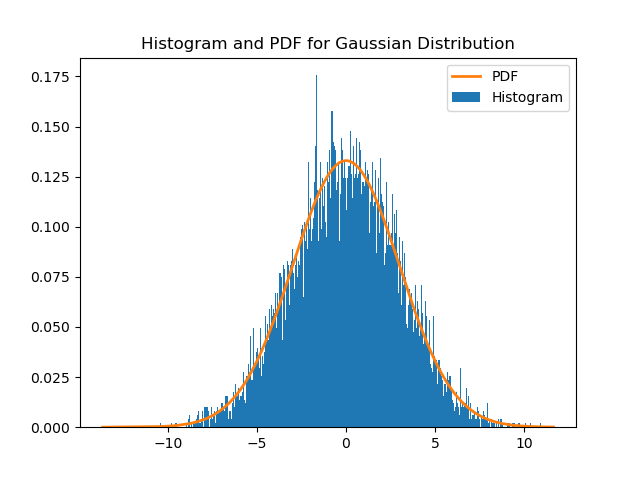
\includegraphics[scale=1]{Q6a.png}
\caption{Histogram and PDF for Gaussian Distribution}
\end{figure}
\end{center}

Inference-
- The values obtained using the CDF inverse have a Gaussian distribution, and we can see the histogram of the distribution matches the PDF.

\pagebreak


\part B
\\
For Rayleigh density with $\sigma=1$ with:\\
* PDF = $f_X(x)=\frac{x}{\sigma^2}e^{-\frac{x}{2\sigma^2}}$\\ 
* CDF = $F_X(x)=1-e^{-\frac{x}{2\sigma^2}}$\\
* Inverse of CDF = $F_X^{-1}(x)=\sigma\sqrt{-2ln(1-x)}$\\
\\
\\
The graph obtained is:
\begin{center}
\begin{figure}[hbtp]
\centering
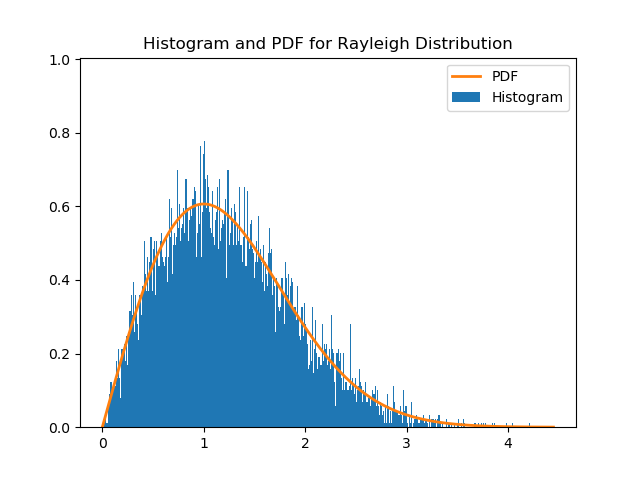
\includegraphics[scale=1]{Q6b.png}
\caption{Histogram and PDF for Rayleigh Distribution}
\end{figure}
\end{center}

Inference-
- The values obtained using the CDF inverse have a Rayleigh distribution, and we can see the histogram of the distribution matches the PDF.

\pagebreak

\part C
\\
For Exponential density with $\lambda$=1.5, we have:\\
* PDF = $f_X(x)=\lambda e^{-\lambda x}$\\
* CDF = $F_X(x)=1-e^{-\lambda x}$\\
* Inverse of CDF = $F_X^{-1}(x)=\frac{-ln(1-x)}{\lambda}$\\ 
(The standard deviation $\sigma=\frac{1}{\lambda}$).
\\
\\
The graph obtained is:
\begin{center}
\begin{figure}[hbtp]
\centering
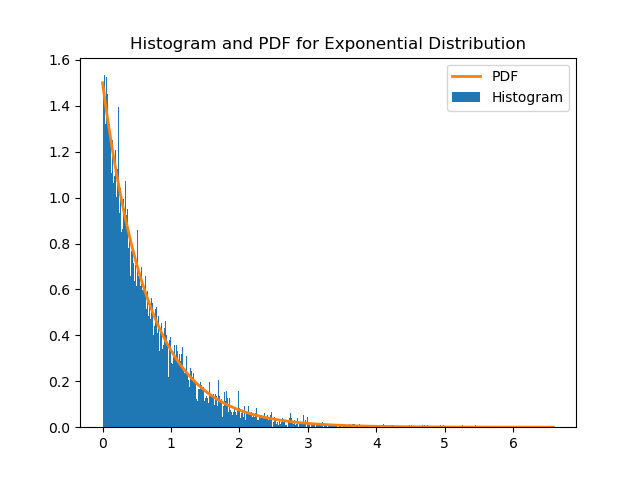
\includegraphics[scale=1]{Q6c.png}
\caption{Histogram and PDF for Exponential Distribution}
\end{figure}
\end{center}
Inference-
- The values obtained using the CDF inverse have an Exponential distribution, and we can see the histogram of the distribution matches the PDF..


\end{homeworkProblem}
\pagebreak

\begin{homeworkProblem}
    Write a function to generate a random number as follows: Every time the function is called, it generates 500 new random numbers from U[0,1] and outputs their sum. \\
    Generate 50,000 random numbers by repeatedly calling the above function, and plot their normalized histogram (with bin-size = 1). What do you find about the shape of the resulting histogram?
    \\
    
    \solution
    \\

I have written the following code in python3 to generate the required graph:
\begin{verbatim}
import matplotlib.pyplot as plt
import numpy as np

def sum500():
  return np.random.random(500).sum()

arr = []
for i in range(50000):
    arr.append(sum500())

plt.hist(arr,density=True,bins=500,label='Histogram')
plt.title('Generated histogram after normalization')
plt.legend()
plt.show()
\end{verbatim}
\\
The graph obtained is:
\begin{center}
\begin{figure}[hbtp]
\centering
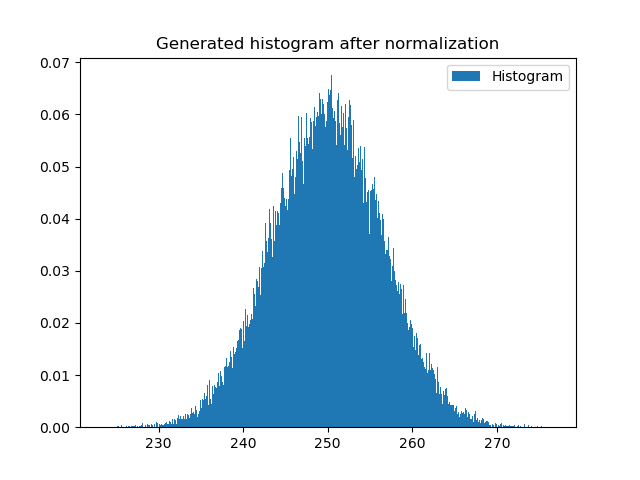
\includegraphics[scale=0.5]{Q7.png}
% \caption{Histogram and PDF for Exponential Distribution}
\end{figure}
\end{center}
    
Observation:\\ 
We can see the distribution in the histogram corresponds to a Gaussian distribution with the peak at 250. This result can be explained using Central Limit Theorem, which states that if you have a population with mean $\mu$ and standard deviation $\sigma$ and take sufficiently large random samples from the population with replacement, then the distribution of the sample means will be approximately normally distributed.\\
% That is, for n independent random variables $X_1,X_2,...,X_n$ with mean $\mu$ and standard deviation $\sigma$, let the resulting random variable be \begin{aligned}
% $Z=\sum_{i=1}^nX_i$
% \end{aligned}. Then, approximately Z\sim{}$N(n\mu,n\sigma^2)$.
\end{homeworkProblem}
%
% Non sequential homework problems
%

% Jump to problem 18

\end{document}
